% !TEX root = ../main.tex
\chapter{Introduction}
The following experiments explore lasers and their applications as well as interference phenomena.

\section{He-Ne Laser}
The common He-Ne-laser consists of a thin (ca. \SI{1}{\milli\meter} in diameter) glass tube filled with a helium-neon gas mixture.
The gas usually is under a pressure of around \SI{100}{\pascal}, where the partial pressures of helium/neon are dependent of the desired wave length of the laser.
At both ends, resonator mirrors are installed with optional Brewster-windows before them.
These Brewster-windows transmit light only of a specific polarisation direction, other directions are mostly reflected.
This means that a laser with Brewster-windows principally emits linear polarized light (more detailed explanations can be found in \autoref{sec:brewster}).

The functioning can be described as follows:
If a high voltage is applied in the filaments, free electrons are created through gas discharge, which can collide with the helium atoms, moving them into an excited state.
The excited helium atoms can stimulate other neon atoms, inducing a population inversion among them.
The term population inversion refers to a situation in which more electrons are in higher states than others.
This process is called \textbf{optical pumping} and is absolutely obligatory for the functioning of the laser.

Changes of state in the neon atoms emit photons by stimulated emission.
These photons are fed back into the system by the resonator and can stimulate other atoms, effectively amplifying emission of photons.

\section{Brewster-angle}\label{sec:brewster}
\begin{figure}[tb]
	\centering
	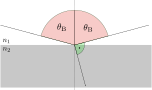
\includegraphics[width=0.8\textwidth]{./img/brewster.pdf}
	\caption[Brewster-angle]{The Brewster-angle}
\end{figure}
When light hits a surface (e.g. glass) it causes dipoles to oscillate inside the material, which radiate and so create reflection and transmission of light.
These dipoles radiate linear polarized light only vertical to their axis of vibration.
If the angle between the reflected and the transmitted light is equal to \SI{90}{\degree}, the intensity of the reflected p-polarized portion disappears, because the dipoles' axis of oscillation is parallel to the direction of transmitted light.
The the s-polarized share, however, is reflected according to Fresnel's law.

By trivial calculations we can show that
\begin{equation}\label{eq:brewster}
	\tan\theta_\text{B}=\frac{n_2}{n_1},
\end{equation}
where $\theta_\text{B}$ denotes the Brewster-angle and $n_2, n_1$ denote the refraction indices of the material and air respectively (assuming the experiment is being condcuted in air).
\section{Fourier Optics}
